% !TEX root = ../../thesis.tex

% \cleardoublepage
% \newpage
% \thispagestyle{plain}
% \mbox{}
% \includepdf{/Users/matthieulapeyre/Documents/phd_thesis/media/thebeast.pdf}
\chapter{Robot morphology: some facinating work} % (fold)




\section{How the morphology can control stuff ?} % (fold)

Once upon a time, in a age where transistor were not here, complex computation was done using mechanical properties.
Using complex mechanisms the very first calculators were fully mechanical (see \figurename~\ref{fig:mechanical_computer}).

The first freely programmable, binary, floating-point, general-purpose mechanical computer in the world was the Z1 constructed by Zuse between 1936 and 1938 (see \figurename~\ref{fig:zuse_z1}).
This "computer" contained approximately 30,000 components and was incredibly sophisticated, making the Z1 suitable for a wide variety of engineering and scientific applications.

The Curta (see \figurename~\ref{fig:curta_calculator}) is a small, hand-cranked digital mechanical calculator introduced by Curt Herzstark in 1948.
It can be used to perform addition, subtraction, multiplication, division, and (with more difficulty) square roots and other operations.
The Curta's design is a descendant of Gottfried Leibniz's Stepped Reckoner and Thomas's Arithmometer, accumulating values on cogs, which are added or complemented by a stepped drum mechanism.
It has an extremely compact design: a small cylinder that fits in the palm of the hand.

Curtas were considered the best portable calculators available until they were displaced by electronic calculators in the 1970s.

\begin{figure}[]
\centering
    \subfloat[][Zuse Z1 (1936)]{\label{fig:zuse_z1}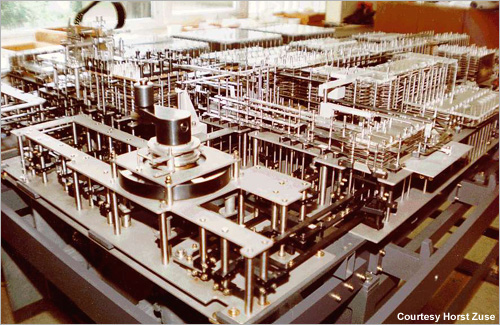
\includegraphics[width=0.42\linewidth]{hist-z1-reconstruct.jpg}}
    \hfil
    \subfloat[][Curta]{\label{fig:curta_calculator}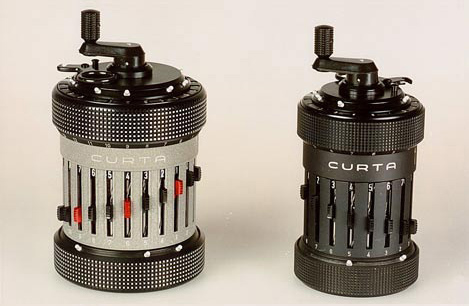
\includegraphics[width=0.42\linewidth]{curta_calculator.jpg}}
    \caption{}
    \label{fig:mechanical_computer}
\end{figure}

% http://www.clivemaxfield.com/diycalculator/popup-h-mechcomp.shtml

% Zuse constructed the Z1 between 1936 and 1938 in his parents' living room in Berlin).
Containing approximately 30,000 components, this purely mechanical computer was incredibly sophisticated.
At that time, mechanical calculators were based on the decimal number system (because that’s the way people thought).
Similarly, when people first started building computers in America (see the discussions on the Mark 1, ENIAC, and so on elsewhere on this site), they initially decided to make them work in decimal, which we now know to be horrendously inefficient.
By comparison, although the Z1 allowed numbers to be input in decimal and displayed its results in decimal, it performed all of its internal calculations in binary (this was to become the standard for all digital computers years later).

% Furthermore, while everyone else was building computers that worked with integer or fixed-point numbers, the Z1 used a binary floating-point system based on a semi-logarithmic representation.
This made it possible to work with very small and very large numbers, thereby making the Z1 suitable for a wide variety of engineering and scientific applications.

% The Z1 was freely programmable in that it could read an arbitrary sequence of instructions from a punch tape.
It featured a control unit that directed operations throughout the machine, a binary floating-point arithmetic unit with sophisticated exception handling, and a 64-word mechanical memory, where each 22-bit word could store arbitrary data and be addressed by both the punch tape and the main control unit.

% The only electromechanical element in the Z1 was a motor, which provided the 1 Hz system clock (there was also a hand crank that could be used to drive the clock manually).
The end result was the first freely programmable, binary, floating-point, general-purpose mechanical computer in the world!



Another great example of how mechanics properties can produce complex behavior is the airplane.
The lift force generated by wings are the resulting of the interaction between a air flux and the physical profil shape of the wing.
Then the Bernouilli law add the necessary magic around to make plane fly (see \figurename~\ref{fig:magic_plane})

\begin{figure}[tb]
    \begin{center}
        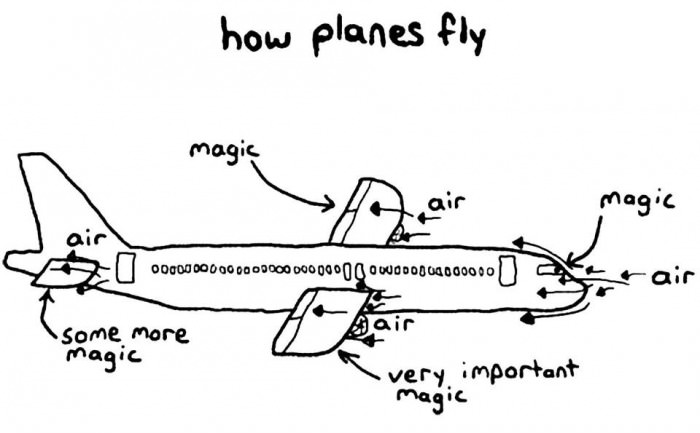
\includegraphics[width=0.8\linewidth]{plane_explanation.jpg}
    \end{center}
    \caption{Caption here}
    \label{fig:magic_plane}
\end{figure}

\begin{figure}[]
\centering
    \subfloat[][]{\label{}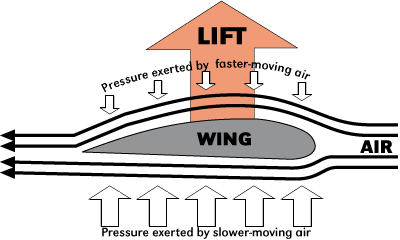
\includegraphics[width=0.56\linewidth]{bernoulli_wing_lift.png}}
    \hfil
    \subfloat[][]{\label{}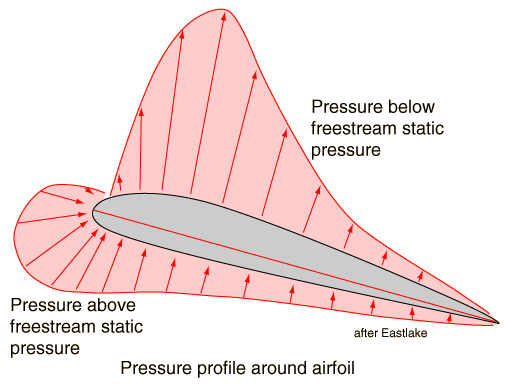
\includegraphics[width=0.42\linewidth]{airfoil_bernouilli.png}}
    \caption{}
    \label{fig:}
\end{figure}

http://tensegritywiki.blogspot.fr/2010/08/mechanism-as-mind-tensegrity-and.html

\section{Robotic} % (fold)
For years, artificial intelligence was only considered through complex computation.
An interesting evolution during the last decade was the emergence of work showing the importance of the actual robot morphology in the robot behavior.

The concept of morphological computation has also been associated to the principle of “ecological balance”, as outlined by Pfeifer et al.
\cite{pfeifer2005new}, which states that there is a balance or task distribution between morphology, materials, control, and interaction with the environment.
For example, morphological computation has been shown to be necessary in order to achieve human-like biped locomotion \cite{matsushita2005locomoting} and the coupling of adequate morphologies with central-pattern generators has been shown to generate robust locomotor behavior \cite{ijspeert2007swimming}\cite{steingrube2010self}.


It has also been shown that the compliance of the body explains the dynamics of walking and running \cite{Geyer2006} and several biped robots such as Athlete Robot \cite{niiyama2010athlete} or BioBiped1 \cite{radkhah2011concept} were designed using compliant actuator or elastic material.
These robots showed interesting hopping and running behavior while using less power actuator than common humanoid robot such as Asimo or HRP-2.

Among all robots designed to explore morphological computation and compliant body only few allow to explore physical interaction such as Kenshiro \cite{Asano2012} or Acroban which the compliant structure of its vertebral column and legs was shown to permit a self-organized physical human-robot interface allowing non-expert users to lead the robot by the hand \cite{Ly2011bio}\cite{Oudeyer2011}.

The morphological properties of these robotic platforms are especially interesting but unfortunately they are difficult and expensive to reproduce by other research laboratories.
Most of the studies made on the humanoid robot locomotion in the past 30 years~\cite{park1998biped}~\cite{aoi2005locomotion}~\cite{park1998biped} mainly focus on tackling the challenge of biped walking through the active control of the whole robot dynamics using technics such as ZMP control~\cite{vukobratovic2004zero} requiring very precise and high torque actuation~\cite{akachi2005development}.

The properties of the robot morphology have shown interesting results for robust locomotion, for instance the hexapod robot Rhex~\cite{saranli2001rhex}.
Still, it is surprising that only few explored the challenge of biped locomotion through the study of the role of morphology.
One can cite the work of Chandana Paul and Josh C.Bongard~\cite{paul2001road} and Ken Endo~\cite{endo2002co} which have explored evolutionary optimization on robot morphology to achieve stable biped locomotion.
They have showed a strong impact of the morphology on the walking behavior and were able to reduce the complexity of the controller by finding good mechanical properties (limbs length and mass distribution).
It has also been shown that human morphological properties such as the compliance of the body explains the dynamics of walking and running \cite{Geyer2006} while experiments made by Kojiro Matsushita~\cite{matsushita2005locomoting} show that an adequate morphology is needed if one is interested in natural looking kind of locomotion.


The role of morphology in robot biped locomotion has been particularly explored through the research on passive dynamic walkers~\cite{wisse2007passive}.
The most famous example concerns the Tad MacGeer's work~\cite{mcgeer1990passive}.
Thanks to the understanding of the intrinsic dynamics of its structure, McGeer has managed to create a 2D biped robot capable of producing several steps without any controller or motor.
The only control of this robot is obtained through the interaction between the intrinsic inertia of the structure and gravity.

\begin{figure}[]
\centering
    \subfloat[][Tad McGeer with his prototypes]{\label{fig:tad_mcgeer}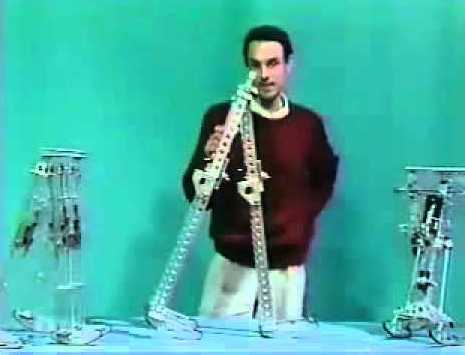
\includegraphics[width=0.49\linewidth]{tad_mcgeer.jpg}}
    \hfil
    \subfloat[][Passive walker robot]{\label{fig:mcgeer_walker}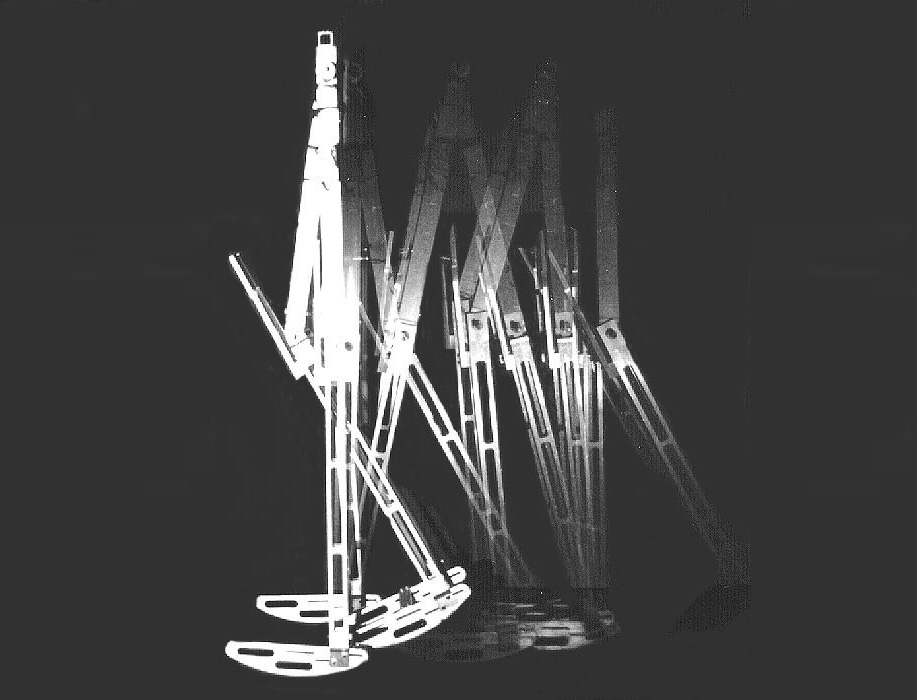
\includegraphics[width=0.49\linewidth]{mcgeer_walker.jpg}}
    \caption{}
    \label{fig:mcgeer_work}
\end{figure}

This work has been pursued with the apparition of semi-passive walker combining both specific passive properties and low power actuation to increase their robustness~\cite{Anderson2005}.
We can note the work of Collins~\cite{collins2005bipedal} which explored the case of semi-passive 3D biped robot.
Its morphology is based on particular mass distribution, knee locking, round feet and springs on the legs to generate an efficient walking gait while keeping its lateral and frontal balance.
The concept of 3D semi-passive robot has been pushed even further with the realization of a complete humanoid robot with trunk, arms and head: the robot Denise~\cite{wisse2005three} and Flame presented in~\cite{Hobbelen2008}.

Several studies have also explored the role of the foot and ankle morphology for biped walking on both human~\cite{Adamczyk2006}~\cite{Hughes1990} and robot~\cite{hobbelen2005ankle}~\cite{Davis2010}.
However, to our best knowledge no research has focused on the role of the thigh for biped locomotion.
While the HRP-4C~\cite{kaneko2009cybernetic} and Kenshiro humanoid~\cite{nakanishi2013design} robot seem to visually have a morphology design close to the thigh shape of Poppy, they did not study, in the associated scientific papers the role of this shape on the dynamic of their humanoid robot.
Most of the studies made on the humanoid robot locomotion in the past 30 years~\cite{park1998biped}~\cite{aoi2005locomotion}~\cite{park1998biped} mainly focus on tackling the challenge of biped walking through the active control of the whole robot dynamics using technics such as ZMP control~\cite{vukobratovic2004zero} requiring very precise and high torque actuation~\cite{akachi2005development}.

Regarding the role of morphology in biped locomotion, one of the first famous example concerns the work of Tad MacGeer on passive dynamic walkers \cite{mcgeer1990passive}.
Thanks to the understanding of the intrinsic dynamics of its structure, McGeer has managed to create a 2D biped robot capable of producing several steps without any controller or motor.
The only control of this robot is due to the interaction between the intrinsic inertia of the structure and gravity.
This work has been pursued by those of Collins \cite{collins2001three} and Tedrake \cite{Tedrake2004}  who perfected the concept to make 3D walkers possible and over longer distances.
The structure of its robot has its own dynamic that allow it to self-stabilize and maintain a walking motion.



\subsection{Passive dynamic walkers} % (fold)



\begin{figure}[]
    \begin{center}
        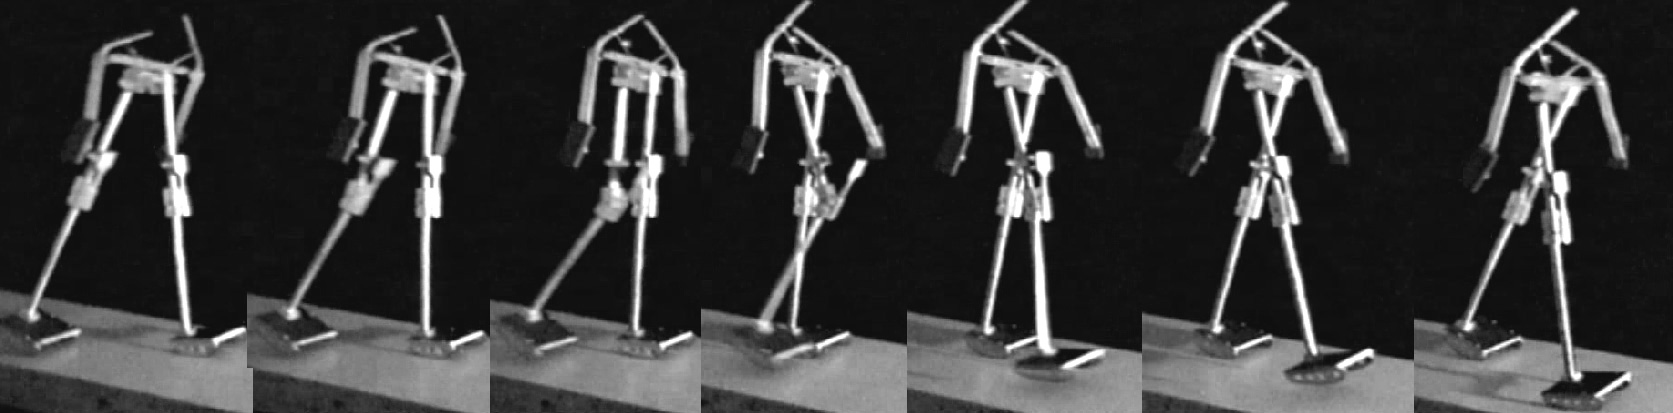
\includegraphics[width=0.99\linewidth]{cornell_biped_series.jpg}
    \end{center}
    \caption{Caption here}
    \label{fig:figure1}
\end{figure}

\begin{figure}[]
    \begin{center}
        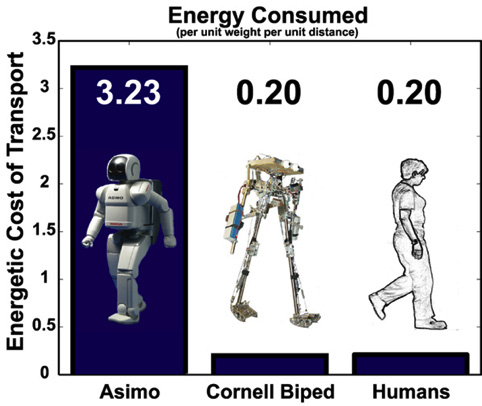
\includegraphics[width=0.6\linewidth]{comparison_cost_transport.jpg}
    \end{center}
    \caption{Caption here}
    \label{fig:figure1}
\end{figure}



\section{Complex emergent behavior} % (fold)


\begin{figure}[]
\centering
    \subfloat[][]{\label{}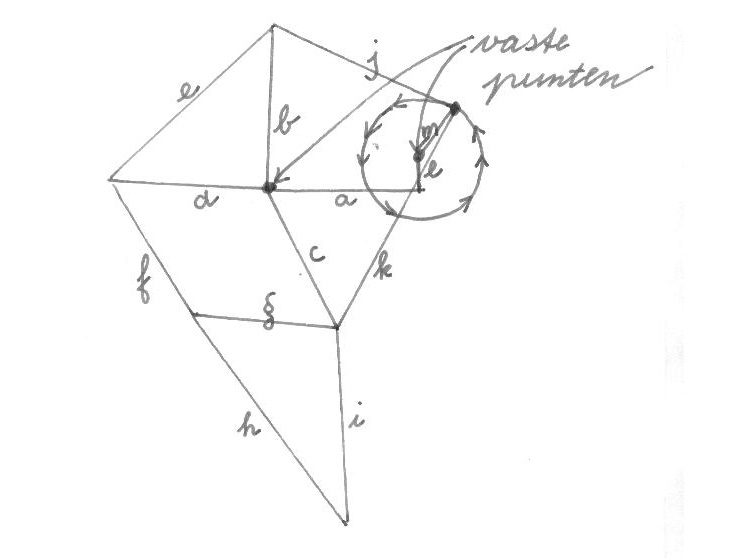
\includegraphics[width=0.32\linewidth]{strandbeest_theory.jpg}}
    \hfil
    \subfloat[][]{\label{}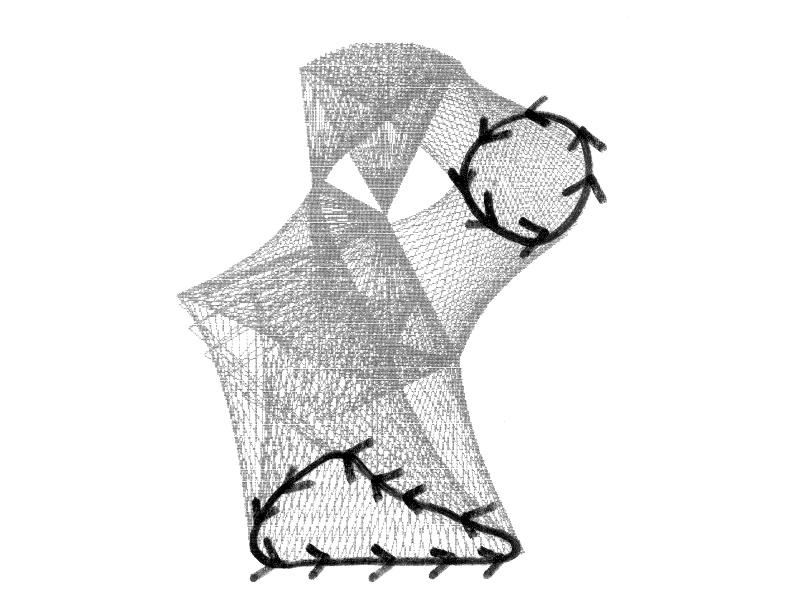
\includegraphics[width=0.32\linewidth]{strandbeest_motion.jpg}}
    \hfil
    \subfloat[][]{\label{}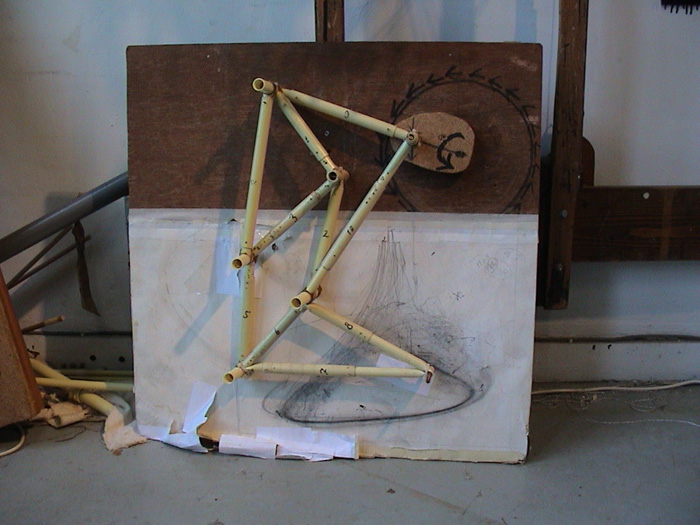
\includegraphics[width=0.32\linewidth]{strandbeest_leg_element.jpg}}
    \caption{}
    \label{fig:}
\end{figure}


\begin{figure}[]
    \begin{center}
        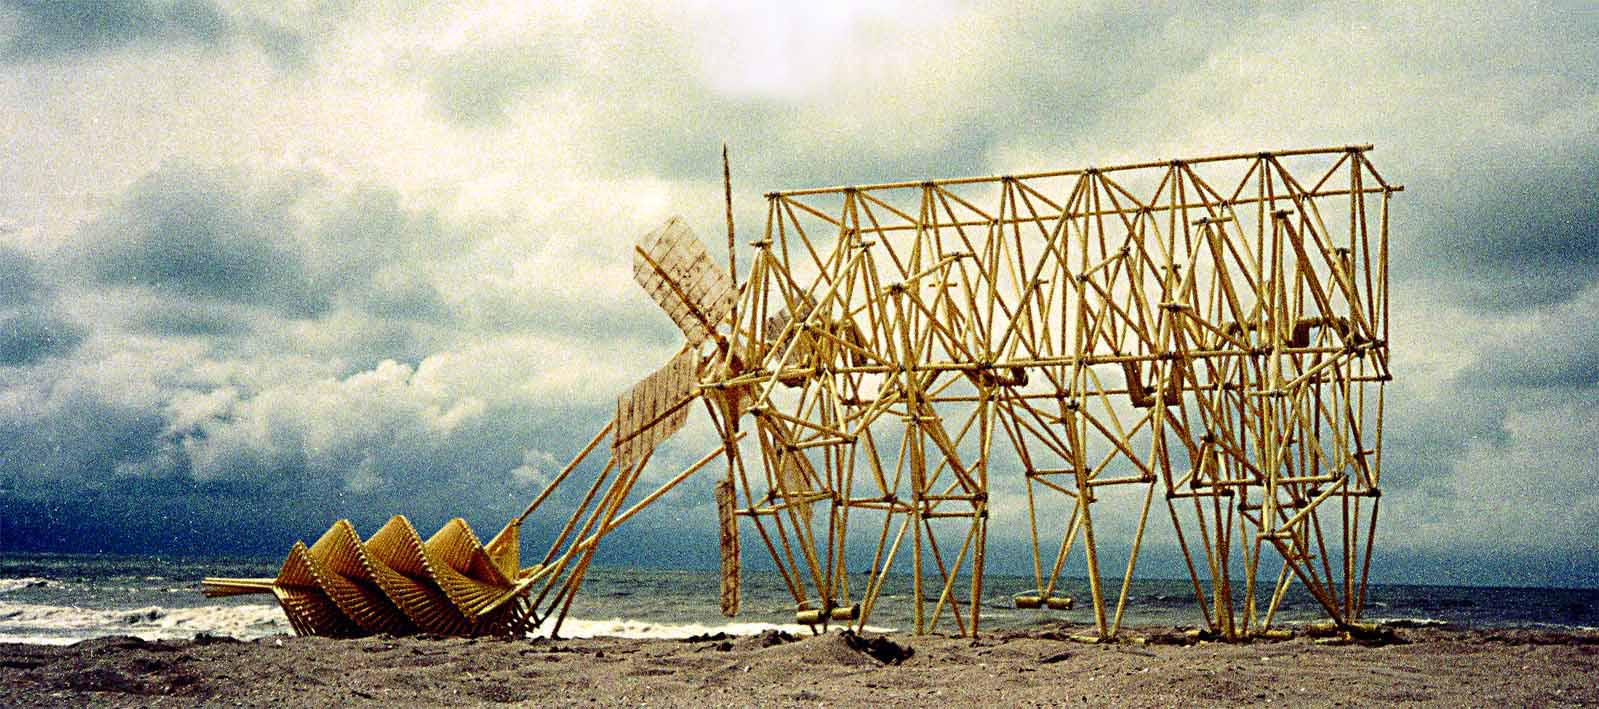
\includegraphics[width=0.99\linewidth]{theo_jansen_beast.jpg}
    \end{center}
    \caption{Caption here}
    \label{fig:figure1}
\end{figure}










\subsection{Locomotion} % (fold)

\subsection{Robustness} % (fold)


\section{Morphology and cognition} % (fold)

\subsection{Data filter} % (fold)

exemple de l'oreille

\subsection{Control stuff} % (fold)

La compliance c'est chouette


Scientific study of the role of morphology in sensorimotor control and cognition: in Robotics (McGeer, Pfeifer and co.), in relation with Cognitive Science (e.g.
http://www.pyoudeyer.com/IEEETAMDOudeyer10.pdf ) and animals (e.g.
work of Robert Full)

\textbf{Object}: In this chapter, we will present a review of different research which has already explored the role of the mophology


\textbf{Conclusion}: The body can definitely take in charge a part of the complexity.
And we need to continue studying it by EXPERIMENTATIONS.
Even if simulator can be complementary.
% chapter exploration_of_the_morphology_role (end)

